\documentclass[border=10pt]{standalone}
\usepackage[svgnames]{xcolor}
\usepackage{amsmath}
\usepackage{pgfplots}
\pgfplotsset{compat=newest}
\usepackage[sfdefault]{FiraSans}
\usepackage{FiraMono}
\renewcommand*\familydefault{\sfdefault}
\begin{document}
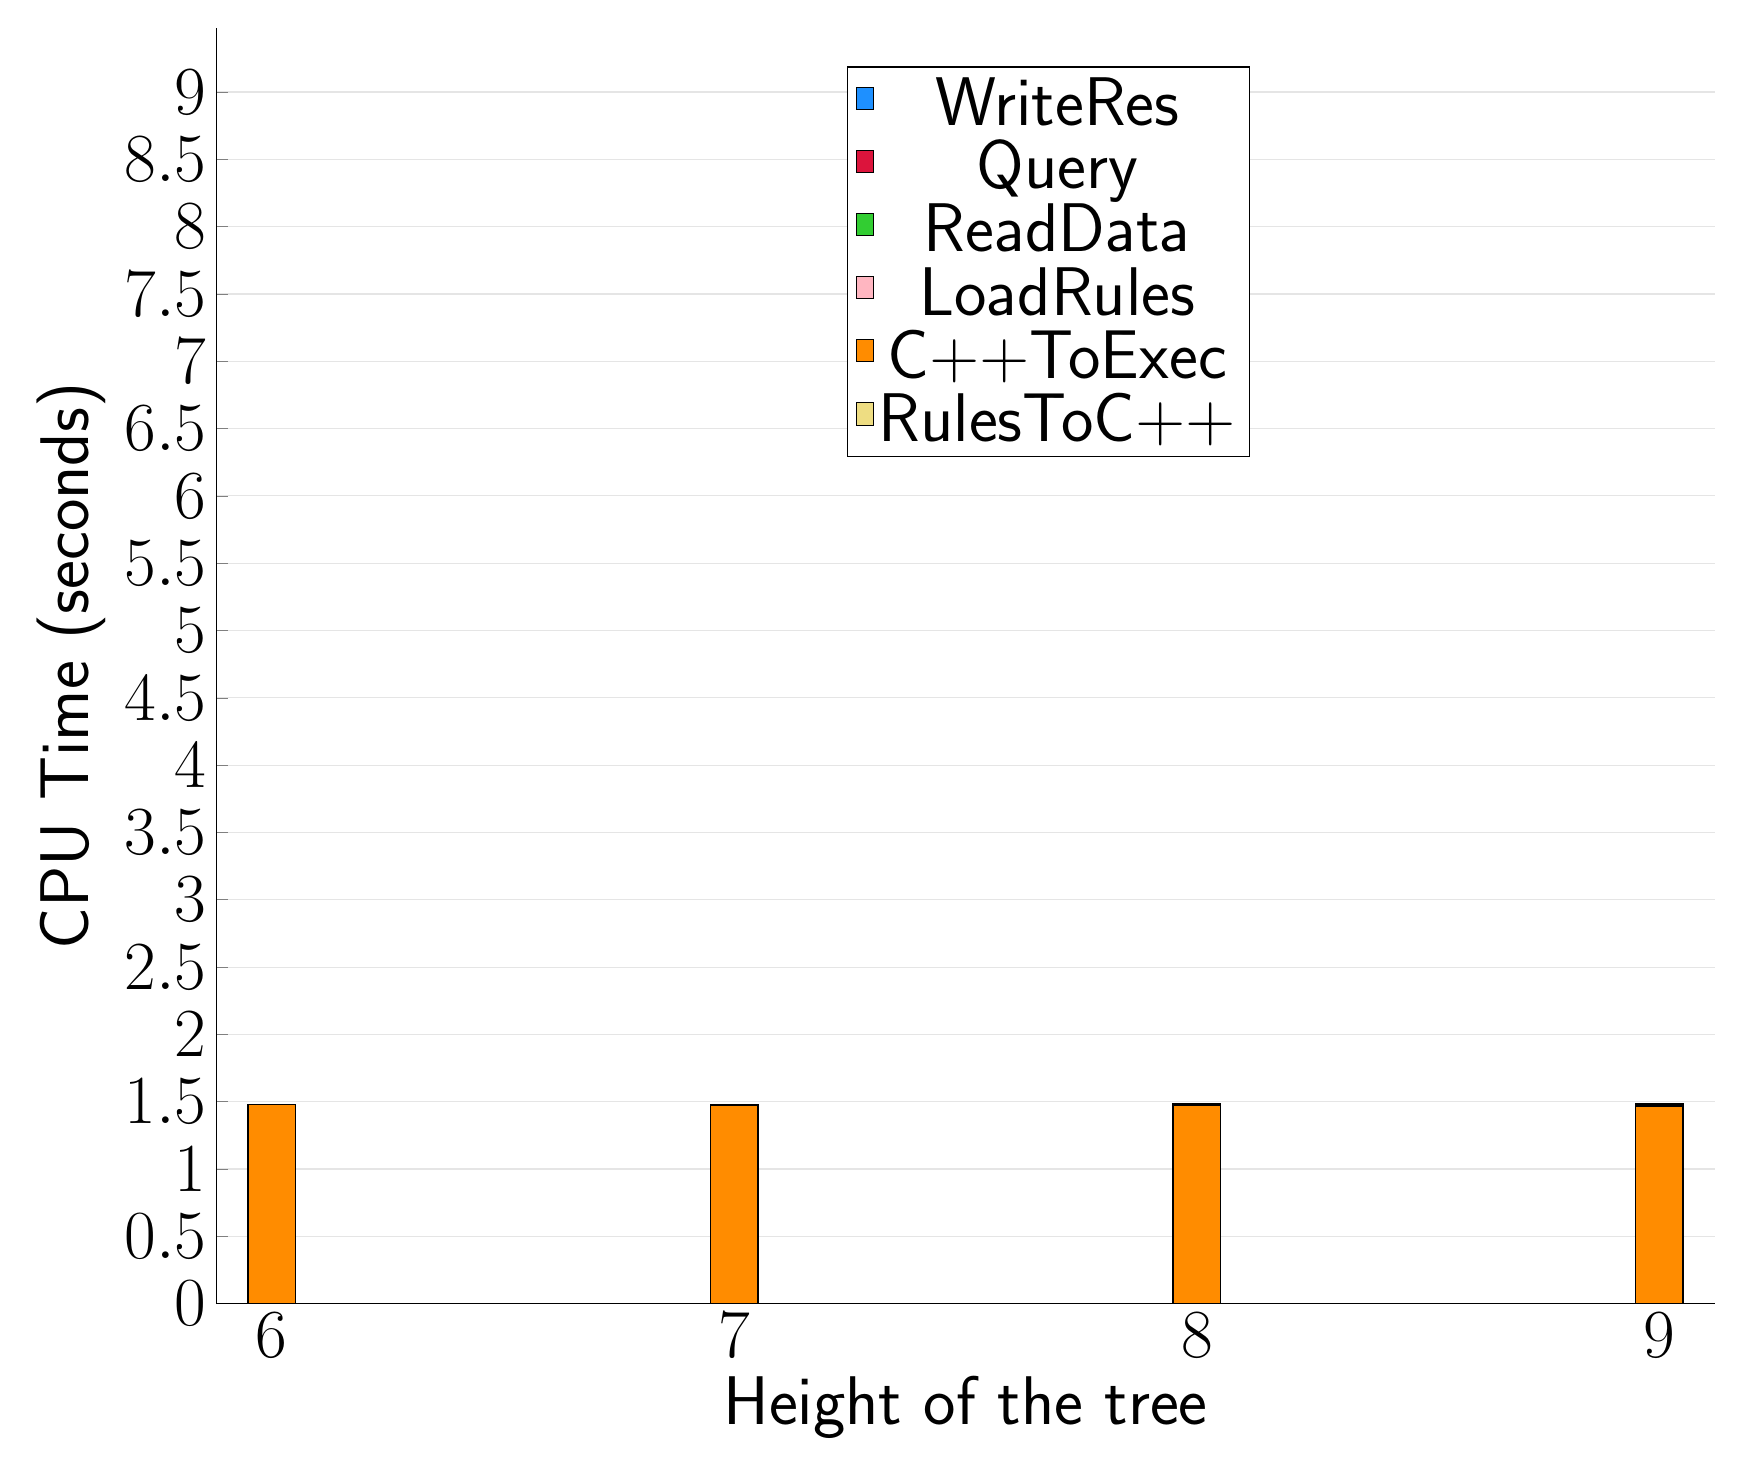
\begin{tikzpicture}
\begin{axis}[
   ybar stacked,
   width=1.7\textwidth,
   bar width=0.6cm,
   ymajorgrids, tick align=inside,
   major grid style={draw=gray!20},
   xtick=data,
   ymin=0, ymax=9.474,
   axis x line*=bottom,
   axis y line*=left,
   enlarge x limits=0.04,
   legend style={
       at={(0.69, 0.97)},
       anchor=north east,
       legend columns=1,
       font=\Huge,
   },
   ylabel={CPU Time (seconds)},
   xlabel={Height of the tree},
   label style={font=\Huge},
   tick label style={font=\Huge},
]
\addlegendimage{fill=DodgerBlue, draw=black, line width=0.2pt}
\addlegendentry{WriteRes}
\addlegendimage{fill=Crimson, draw=black, line width=0.2pt}
\addlegendentry{Query}
\addlegendimage{fill=LimeGreen, draw=black, line width=0.2pt}
\addlegendentry{ReadData}
\addlegendimage{fill=LightPink, draw=black, line width=0.2pt}
\addlegendentry{LoadRules}
\addlegendimage{fill=DarkOrange, draw=black, line width=0.2pt}
\addlegendentry{C++ToExec}
\addlegendimage{fill=LightGoldenrod, draw=black, line width=0.2pt}
\addlegendentry{RulesToC++}
\addplot +[fill=LightGoldenrod, draw=black, line width=0.55pt] coordinates {
(6, 0.0)
(7, 0.0)
(8, 0.0020000000000000005)
(8, 0.0020000000000000005)
(8, 0.0020000000000000005)
(9, 0.0)
(9, 0.0)
(9, 0.0)
(9, 0.0)
(9, 0.0)
};
\addplot +[fill=DarkOrange, draw=black, line width=0.55pt] coordinates {
(6, 1.478)
(7, 1.472)
(8, 1.472)
(8, 1.4739999999999998)
(8, 1.474)
(9, 1.47)
(9, 1.47)
(9, 1.468)
(9, 1.476)
(9, 1.468)
};
\addplot +[fill=LightPink, draw=black, line width=0.55pt] coordinates {
(6, 0.0001662)
(7, 0.00019020000000000002)
(8, 0.0001866)
(8, 0.000165)
(8, 0.00017600000000000002)
(9, 0.0001672)
(9, 0.0001658)
(9, 0.000172)
(9, 0.000175)
(9, 0.00017299999999999998)
};
\addplot +[fill=LimeGreen, draw=black, line width=0.55pt] coordinates {
(6, 0.0006652)
(7, 0.0009094)
(8, 0.0013333999999999998)
(8, 0.0014372)
(8, 0.0014437999999999999)
(9, 0.0023518)
(9, 0.0023474000000000004)
(9, 0.0023566)
(9, 0.0024657999999999998)
(9, 0.0024214)
};
\addplot +[fill=Crimson, draw=black, line width=0.55pt] coordinates {
(6, 0.0005874000000000001)
(7, 0.001362)
(8, 0.0028692)
(8, 0.002977)
(8, 0.0031130000000000003)
(9, 0.0058172)
(9, 0.0060508)
(9, 0.006560400000000001)
(9, 0.0068588)
(9, 0.006729399999999999)
};
\addplot +[fill=DodgerBlue, draw=black, line width=0.55pt] coordinates {
(6, 0.000658)
(7, 0.0009586000000000001)
(8, 0.0014204)
(8, 0.001483)
(8, 0.0014906000000000001)
(9, 0.0018993999999999997)
(9, 0.0021574000000000003)
(9, 0.001954)
(9, 0.002155)
(9, 0.0022562000000000003)
};
\end{axis}
\end{tikzpicture}

\end{document}
